
\documentclass[ms.tex]{subfiles}
\begin{document}

\section{Methods}
\label{sec:methods}

\begin{itemize}

	\item We are interested in applying one-zone GCE models to dwarf galaxies
	and determining best-fit parameters.
	We begin by providing background on one-zone models, and then we select
	a parametrization from which we draw a fiducial mock stellar sample.
	We then use these data to introduce our fitting method.

\end{itemize}

\subsection{One-Zone Models of Galactic Chemical Evolution}
\label{sec:methods:onezone}

\begin{itemize}

	\item The fundamental assumption of one-zone models is that newly produced
	metals mix instantaneously throughout the star forming gas reservoir.
	This approximation is valid as long as the mixing time-scale is negligible
	compared to the depletion time-scale (i.e. the average time an fluid
	element remains in the ISM before getting incorporated into new stars or
	ejected in an outflow).
	Based on the observations of~\citet{Leroy2008},~\citet*{Weinberg2017}
	calculate that characteristic depletion times can range from~$\sim$500 Myr
	up to~$\sim$10 Gyr for conditions in typical star forming disc galaxies.
	With the short length-scales and turbulent velocities of dwarf galaxies,
	instantaneous mixing should be a good approximation.

	\begin{itemize}
		\item {\color{red}
		If there's an observational reference of metal-mixing in the dwarf
		galaxy regime - specifically if the scatter in the~\afe-\feh~plane is
		dominated by observational uncertainty - Evan Kirby would probably be
		the one to know about it.
		If not, this would be a good thing to call out as a good observational
		test of the validity of the one-zone approximation.
		}
	\end{itemize}

	\item The assumption of instantaneous mixing eliminates the need for
	spacial information, reducing GCE to a system of coupled
	integro-differential equations which can be solved numerically.

	\item At a given moment in time, gas is added to the interstellar medium
	(ISM) via inflows and recycled stellar envelopes and is taken out of the
	ISM via outflows and new stars.
	This gives rise to the following differential equation describing the
	evolution of the gas-supply:
	\begin{equation}
	\dot{M}_\text{g} = \dot{M}_\text{in} - \dot{M}_\star - \dot{M}_\text{out}
	+ \dot{M}_\text{r},
	\end{equation}
	where~$\dot{M}_\text{in}$ is the infall rate,~$\dot{M}_\star$ is the star
	formation rate (SFR),~$\dot{M}_\text{out}$ is the outflow rate,
	and~$\dot{M}_\text{r}$ is the return of stellar envelopes from previous
	generations of stars.

	\begin{itemize}
		\item There are various prescriptions for outflows in the literature.
		Some authors~\citep[e.g.][]{Andrews2017, Weinberg2017} assume a linear
		proportionality between the two:
		\begin{equation}
		\label{eq:eta}
		\dot{M}_\text{out} \equiv \eta\dot{M}_\star.
		\end{equation}
		Recently,~\citet{delosReyes2022} constrained the evolution of the
		Sculptor dwarf spheroidal galaxy with a linear proportionality between
		the SFR and the SN rate~$\dot{N}_\text{II} + \dot{N}_\text{Ia}$.
		For modelling the Milky Way, some authors neglect outflows, arguing
		that they do not signicantly alter the chemical evolution of the
		disc~\citep[e.g.][]{Spitoni2019, Spitoni2021}.
		In our mock sample and in our fits to the GSE and the Sagitarrius dSph,
		we assume the linear proportionality given by equation~\refp{eq:eta}.
		Our fitting routine, however, is easily extended to the parametrization
		of~\citet{delosReyes2022}, and if outflows are to be neglected, one can
		simply take~$\eta = 0$ in their fit.
	\end{itemize}


\end{itemize}

\subsection{A Fiducial Mock Sample}
\label{sec:methods:fiducialmock}

\begin{figure*}
\centering
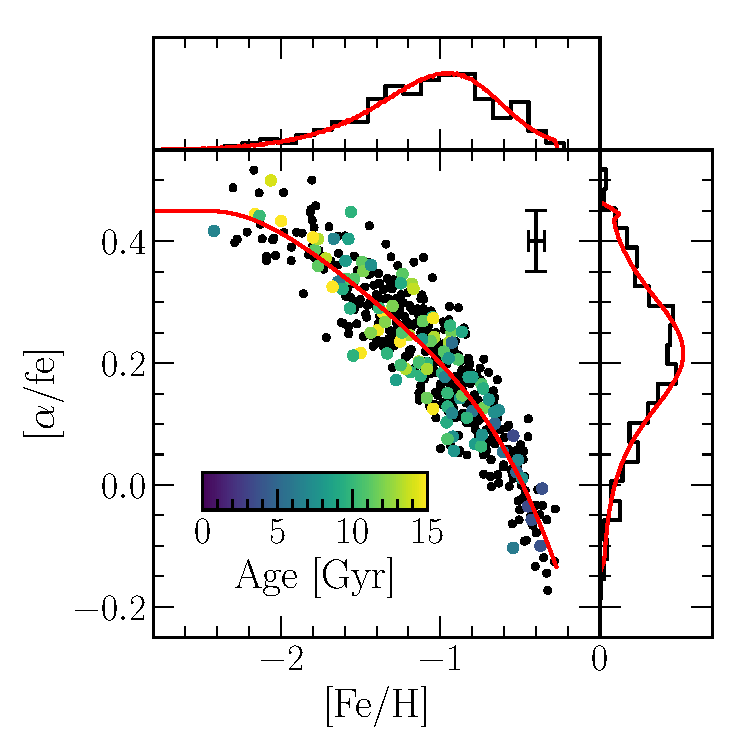
\includegraphics[scale = 0.5]{fiducial_mock_afe_feh.pdf}
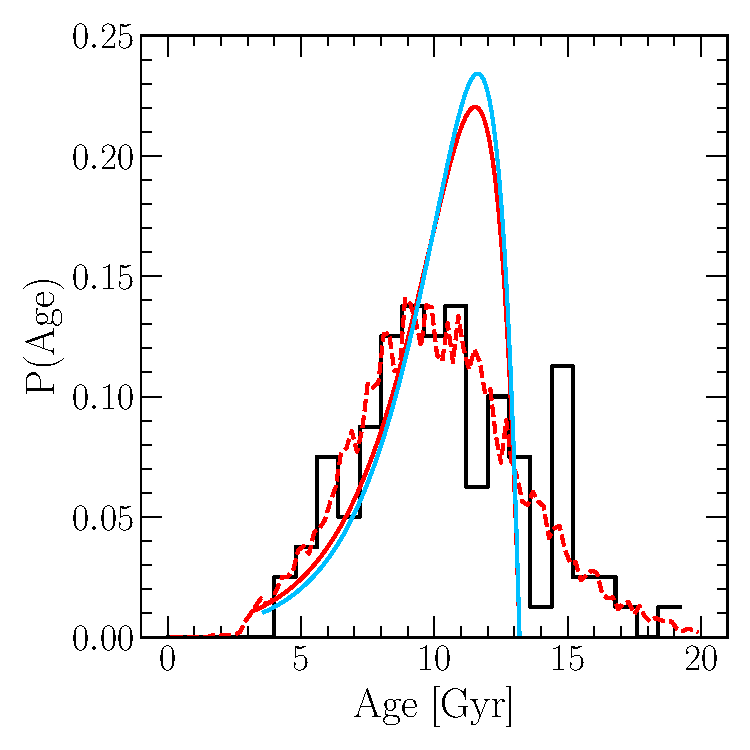
\includegraphics[scale = 0.42]{fiducial_mock_agedist.pdf}
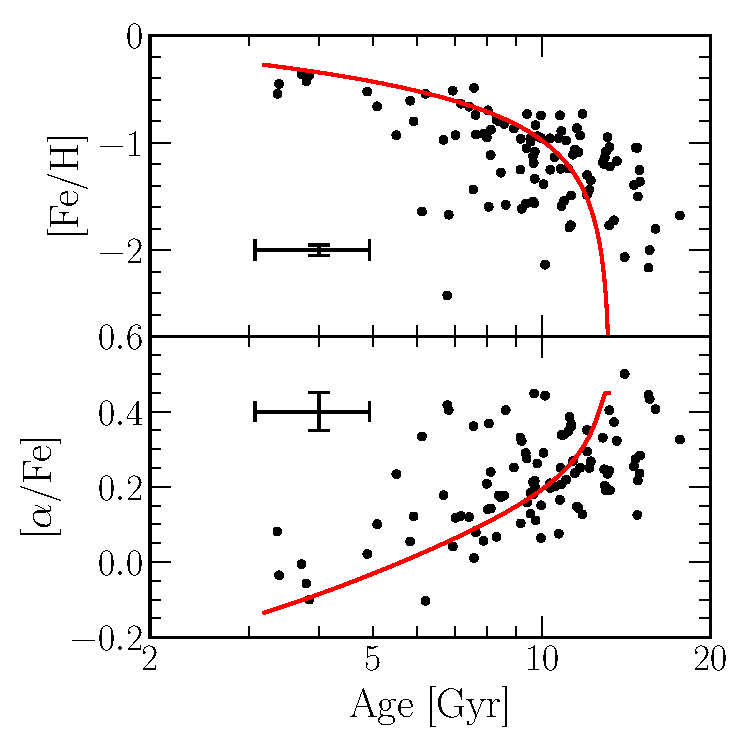
\includegraphics[scale = 0.42]{fiducial_mock_amr.pdf}
\caption{
\textbf{Left}: Our fiducial mock sample in the~\afe-\feh~plane.
There are~$N = 500$ stars with abundance uncertainties
of~$\sigma(\feh) = \sigma(\afe) = 0.05$ as indicated by the errorbar.
$N = 100$ of the stars have age information available with an artificial
uncertainty of~$\sigma(\log_{10}(\text{age})) = 0.1$ as indicated by the
colorbar.
The red line denotes the evolutionary track in the gas-phase from the one-zone
model that generated the mock.
On the top and right, we show the marginalized distributions
in~\afe~and~\feh, with red lines denoting the known distribution.
\textbf{Center}: The mock (black, binned) and known (red) age distributions.
The dashed red line indicates the age distribution that is obtained by sampling
$N = 10^4$ rather than $N = 500$ stars and assuming the same age uncertainty
of~$\sigma(\log_{10}(\text{age})) = 0.1$.
\textbf{Right}: The age-\feh~(top) and age-\afe~(bottom) relation for the mock
sample, with artificial uncertainties denoted by the error bars on each panel.
The red lines denotes the known relations for the gas-phase.
}
\label{fig:fiducialmock}
\end{figure*}


\subsection{The Fitting Method}
\label{sec:methods:fitting}

\begin{itemize}

	\item Introduce a new algorithm that fits the track itself to
	the~\feh~and~\afe~abundances of individual stars as opposed to binning the
	data and fitting the distribution.
	Though we use chemical abundances as our chief observational quantity, this
	procedure is highly generic and should in principle be applicable in any
	region of parameter space where there is intrinsic variation in the density
	of data points (e.g. isochrones in stellar evolution).

	\item We make use of~\mc~\cite{Foreman-Mackey2013} to run Markov Chain
	Monte Carlo (MCMC) fits of parameters in one-zone models of chemical
	evolution.
	At each step in parameter space,~\mc~makes a call to the~\texttt{Versatile
	Integrator for Chemical Evolution}~\citep[\vice;][]{Johnson2020,
	Griffith2021, Johnson2021} to compute the predicted abundances for that
	selection of parameters.
	We then compute the likelihood function $L(d|m)$ according to the following
	procedure.

	\item For a given realization of a one-zone model with known parameters~$m$
	and one-zone model predictions~$\mu$ = (\feh,~\afe,~\logage), the
	likelihood of the data given the model is equal to the product of the
	likelihoods of each individual data point:
	\begin{subequations}\begin{align}
	L(d|m) &= \prod_i L(d_i|m)
	\\
	\implies \ln L(d|m) &= \sum_i \ln L(d_i|m).
	\end{align}\end{subequations}
	However, for a given model~$m$, there is no guaranteed way of knowing
	which point~$m_j$ along the computed~\afe-\feh~track should correspond to
	some data point~$d_i$.
	We therefore marginalize over the entire track for every data point~$d_i$
	by summing the likelihoods from all~$m_j$ model vectors:
	\begin{subequations}\begin{align}
	L(d_i|m) &= \sum_j L(d_i|m_j)
	\\
	\implies \ln L(d|m) &= \sum_i \ln \left(\sum_j L(d_i|m_j)\right)
	\end{align}\end{subequations}

	\item We relate the data point~$d_i$ and the model point~$m_j$ with the
	relation~$L(d_i|m_j) \propto e^{-\chi^2/2}$ with
	$\chi^2 = \Delta_{ij}C_i^{-1}\Delta_{ij}^T$, where
	$\Delta_{ij} = \mu_{i,\text{data}} - \mu_{j,\text{model}}$ (i.e. the
	difference between a pair of data and model vectors) and $C_i^{-1}$ is the
	inverse covariance matrix of the~$i$th data point.

	\item Chemical evolution tracks, however, have real, intrinsic variations
	in the density of points along the track.
	In one case, a high density of data points may simply reflect the fact that
	the model vector~$\mu_{j,\text{data}}$ is not far from the vector from the
	previous timestep~$\mu_{j - 1,\text{data}}$.
	In another case, a high density of data points may reflect the fact that
	the star formation rate was high when the galaxy was passing through some
	region of parameter space.
	The density of points in the data may also vary because of non-uniform
	sampling.


\end{itemize}

\end{document}
